\documentclass[10pt,a4paper]{article}
% Libraries
\usepackage[utf8]{inputenc} % [utf8] for linux, latin1 for windows
\usepackage[french]{babel} %\usepackage[english]{babel}
\usepackage{fullpage}
\usepackage{amsmath}
\usepackage{amsfonts}
\usepackage{amssymb}
\usepackage{graphicx} 
\usepackage{longtable}

\usepackage{listings}
\usepackage{algorithmic}
\usepackage{float}

\usepackage[center]{caption}
\usepackage{subcaption}

%\usepackage{calc}
\usepackage{amsthm}
%\usepackage[usenames,dvipsnames]{xcolor}
%\usepackage{tikz}
%\usepackage[all]{xy}

\usepackage{hyperref} %[hidelinks]
\usepackage[usenames,dvipsnames]{color}
\hypersetup{
  colorlinks   = true, %Colours links instead of ugly boxes
  urlcolor     = Blue, %Colour for external hyperlinks
  linkcolor    = Blue, %Colour of internal links
  citecolor   = Blue %Colour of citations
}

% To add a word in the links maded by hyperref
% but cleveref goes "laster" than hyperref
\usepackage[nameinlink,noabbrev, french]{cleveref}

% Must be after hyperref
\usepackage{algorithm}

% Pour ordonner les citations etc
\usepackage{cite}


\newtheorem{prop}{Proposition}[section]
\newtheorem{theorem}{Theorem}[section]
\newtheorem{lemma}{Lemma}[section]
\newtheorem{definition}{Definition}[section]
\newtheorem{requirement}{Requirement}[section]
\newtheorem{remark}{Remark}[section]
\newtheorem*{remarks}{Remarks}
\newtheorem{hypothesis}{Hypothesis}[section]
\newtheorem{example}{Example}

\newtheorem{axiom}{Axiome}[section]
\renewcommand{\theaxiom}{\Roman{axiom}} %\renewcommand{\theaxiom}{\thechapter.\thesection.\arabic{axiom}}

\setcounter{secnumdepth}{3}

\author{Jean-Baptiste Lespiau et Charles Thin}
\title{La méthode B : une méthode formelle de développement logiciel}
\date\today


\usepackage{wrapfig}

\newcommand{\Bequal}{\mathrel{\widehat{=}}}

%\renewcommand{\thechapter}{\Roman{chapter})}
%\renewcommand{\thesection}{\Roman{section}} %Alph
%\renewcommand{\thesubsection}{\arabic{subsection})}
%\renewcommand{\thesubsubsection}{\alph{subsubsection})}
%\renewcommand{\theparagraph}{\engrec{paragraph})}
\begin{document}
\maketitle

\begingroup
\hypersetup{hidelinks}
\tableofcontents
\endgroup


\newpage

\begin{abstract}
La méthode B, inventé par Jean-Raymond Abrial, est une méthode pour spécifier, concevoir et générer du code de systèmes logiciels tout en satisfaisant des contraintes de preuves de propriétés.
Elle est basée sur la logique du premier ordre, la théorie des ensembles de Zermelo-Fraenkel avec l'axiome du choix, le concept de substitutions généralisées et une certaine approche de la complexité (par la définition de machine abstraite, raffinement et d'implémentation).
\end{abstract}

\iffalse
0) Courte intro: on va parler de quoi ?
Schema : Meteor: page 374
Utilisé dans tels projets (Météor etc)

1)[J-B] Théorie des ensembles : OK
+ théorie des relations
Exemples
3)[Charles] Explication des machines abstraites et de tous leurs champs
Définie dans Dossier-Technique page 9
Exemple de la bibliothèque: Cours B Part I 2007
4bis) Preuves
5)[Charles] Raffinement d'une machine abstraite (Dossier Technique page 10)
Rajouter un exemple (commence page 193 de Spécification avec B)
5bis) Obligation de preuves des raffinements
6) Preuves et obligations de preuves
7)[J-B] Implémentation d'un raffinement (définir ce qu'il doit contenir ou non).

A la fin:
Les tableaux pour donner les équivalences entre symboles mathématiques et grammaire.
\fi

\section{Introduction}

La méthode B c'est :
\begin{itemize}
\item une théorie mathématique basée sur la théorie des ensembles et des relations~;
\item une méthode pour spécifier, concevoir et implémenter des logiciels~;
\item un langage~;
\item un ensemble d'outils dont le principal est l'Atelier B\footnote{\url{http://www.methode-b.com/}} (développé par la société ClearSy). Il existe également d'autres produits comme B-Toolkit ainsi que des logiciels libres mais bien moins aboutis (comme B4free\footnote{\url{http://www.b4free.com/}} ou ABTools\footnote{\url{http://sourceforge.net/projects/abtools/}}).
\end{itemize}
~

En particulier, l'Atelier B est entre autres constitué de :
\begin{itemize}
\item un analyseur~;
\item un générateur d'obligation de preuve~;
\item un démonstrateur automatique~;
\item un démonstrateur interactif~;
\item un générateur de code C et Ada~;
\item un gestionnaire de projet...
\end{itemize}

Le formalisme de modélisation s'appuie sur plusieurs concepts : la théorie des ensembles, la logique des prédicats du premier ordre et le langage de substitutions généralisées.

Pour concevoir ce document, nous nous sommes basés sur \cite{behm1999meteor, habrias2006specifications, theBBook, dossierTechnique, VerimagPDF}

\section{Théorie sous-jacente de la méthode B}

La méthode B repose d'abord sur la logique du premier ordre. Une définition formelle des règles de remplacement sont données sur \url{http://www.labri.fr/perso/retore/GeoLog/mementoFOL.pdf} par exemple. Il est important de distinguer une expression d'un prédicat. Un récapitulatif est donné en~\cref{SyntaxPredicatExpression}.

\subsection{Axiomatique ensembliste}

La théorie sous-jacente utilisée provient de la théorie des ensembles de Zermelo-Fraenkel avec axiome du choix (ZFC) dont les axiomes sont présentés en \cref{ZFC}.
Cependant, la théorie des ensembles utilisée dans B est une théorie simplifiée dans le sens où certains axiomes ne sont pas utilisés :
\begin{itemize}
\item Les deux axiomes de  Fraenkel~;
\item L'axiome de la réunion.
\end{itemize}~
De plus, l'axiome de la paire est modifié pour construire une paire ordonnée et non un ensemble. 

Cela donne ainsi l'axiomatique:
\begin{description}
\item[Définition de la paire] $(E, F) \in s \times t \Leftrightarrow E \in s \wedge F \in t$
\item[Ensemble des parties] $s \in \mathbb{P}(t) \Leftrightarrow \forall x (x \in s \rightarrow x \in t)$
\item[Ensemble en compréhension] $E \in \{ x | x \in s \wedge P \} \Leftrightarrow (E \in s \wedge [x:= E] P)$
\item[Égalité d'ensembles] $\forall x (x \in s \Leftrightarrow x \in t) \Rightarrow s = t$
\item[Axiome du choix] $\exists x  (x \in s) \Rightarrow choice(s) \in s$
\item[Axiome de l'infini] Existence d'un ensemble infini nommé BIG
\end{description}

\subsection{Type-checking}

L'idée est que, lors de la preuve d'un prédicat ayant des variables liées à des quantificateurs, les variables liées sont supposées appartenir à un ensemble.
Sans en détailler ici toutes les implications, il est toutefois important de remarquer que l'ajout de ces contraintes de type-checking rend l'ensemble vide typé du type de l'ensemble dont il est le résultat (i.e. $\varnothing = A - A$), et il n'y a donc pas unicité de l'ensemble vide. 

\subsection{Langage de substitution généralisée}

Un triplet $ \{P\}\;S\;\{Q\} $ est à interpréter dans la logique de Hoare de la façon suivante : si la propriété $P$ est vraie et qu'on exécute le code $S$, alors si $S$ termine on a la propriété $Q$. En particulier, si on n'a pas de garantie sur la terminaison de l'instruction $S$ on parle de correction partielle. La propriété $P$ est appelée précondition et $Q$ postcondition. Les axiomes de la logique de Hoare sont donnés en~\cref{Hoare}.

Pour un prédicat $Q$ et une exécution $S$, on définie la plus faible précondition $wp(S, Q)$ (\emph{wp} pour weakest precondition) telle que :
\begin{itemize}
\item $wp(S, Q)$ est une précondition garantissant $Q$  après exécution de $S$ : $ \{ wp(S, Q) \} S \{ Q\}$
\item $wp(S, Q)$  est la plus faible précondition : si $\{ P \} S \{ Q \}$ alors $P \Rightarrow wp(S, Q)$.
\end{itemize}~

En B on utilise la notation $[S]Q$ au lieu de $wp(S, Q)$. On ne traitera pas ici de l'existence de la plus faible précondition mais la preuve se fait par induction structurelle\footnote{On pourra aller voir \url{http://www.lsv.ens-cachan.fr/~haddad/courstdagreg.pdf} pour une peuve complète.}. Voici la définition de certaines substitutions généralisées\footnote{La boucle n'a pas été définie par exemple.} :
\begin{description}
\item[Substitution simple] ~

$[ x := E ]P \Leftrightarrow P[E/x]$ où $P[E/x]$ est le prédicat $P$ où toutes les occurrences libres de $x$ (i.e. qui ne sont pas sous le contrôle d'un quantificateur) ont été remplacé par $E$. En particulier, on a alors $\{ [x := E ]P \} x := E\{ P\}$, par définition même de la plus faible précondition.
\item[Substitution identité]  ~

$[\textsc{skip}]I \Leftrightarrow I$
\item[Substitution séquentielle]  ~

$[S1;S2]P 	\Leftrightarrow [S1]([S2]P)$
\item[Substitution préconditionnée]  ~

$[\textsc{PRE } P \textsc{ THEN } S \textsc{ END}]I \Leftrightarrow P \wedge [S]I$
\item[Substitution conditionnelle]  ~

$[\textsc{IF } Q \textsc{ THEN } S1 \textsc{ ELSE } S2 \textsc{ END}]P \Leftrightarrow (Q \Rightarrow [S1]P) \wedge( (\lnot Q)\Rightarrow [S2]P)$
\item[Substitution gardée]  ~

$[\textsc{SELECT } P \textsc{ THEN } S \textsc{ END}]I \Leftrightarrow P \Rightarrow [S]I$
\item[Substitution de choix binaire indéterministe]  ~

$[\textsc{CHOICE } S \textsc{ OR } T \textsc{ END}]I \Leftrightarrow [S]I \wedge [T ]I$
\item[Substitution de choix non borné indéterministe] ~

$[\textsc{ANY } z \textsc{ WHERE } P \textsc{ THEN } S \textsc{ END}]I \Leftrightarrow \forall x \bullet [S]I$ pour x n'étant pas libre dans I
\end{description}


\subsection{Relations et fonctions}

On note  $ s \leftrightarrow t \Bequal \mathbb{P}(s \times t)$ qui est l'ensemble des relations entre les éléments de $s$ et les éléments de $t$. De plus, une paire ordonnée $(x, y)$ est notée $x \mapsto y$.

\section{Machines abstraites}

\subsection{Description informelle}

La méthode B est fondée sur la notion de \emph{modèle}. Un \emph{modèle} décrit les \emph{opérations} d'un système, ses données entrantes et sortantes et des valeurs (son \emph{état}) et des propriétés sur ces données et valeurs (des \emph{contraintes} ou \emph{invariants}).

Un utilisateur d'un système qui en connaît un modèle peut fournir des données et des valeurs en entrée (i.e. fournir un état du système dans la modélisation actuelle) et observer l'état sortant. Tous ces  éléments (propriétés, données, opérations, état) peuvent être aussi abstraits et généraux que voulu.

L'utilisateur ne connaît rien du fonctionnement interne du système au delà de la précision de son modèle. Ainsi la suite des états internes par lesquels passe la machine lors d'une opération n'est pas accessible à l'utilisateur ayant déclenché l'opération.
\\

En méthode B, ces notions se traduisent dans une \emph{machine abstraite} : c'est exactement l'appellation en méthode B d'un modèle. Une machine abstraite propose et réalise des opérations (c'est une machine) directement implémentables en code logiciel ou non (elle est abstraite).

Notons, d'un point de vue industriel, qu'une machine abstraite représente un ensemble de besoins, d'exigences ou de spécifications de niveau donné. Nous verrons par la suite comment, de même que l'on précise et concrétise des besoins en exigences puis en spécifications de plus en plus précises et de plus en plus proche de l'implémentation, on raffine des machines abstraites jusqu'à des implémentations.

\subsection{Description formelle}

Une machine abstraite c'est :
\begin{itemize}
\item un \textbf{nom}, pour l'appel depuis l'extérieur~;
\item des \textbf{paramètres}, dimensionnant la machine~;
\item des \textbf{contraintes}, sur les paramètres~;
\item un \textbf{état}, composé des valeurs d'un ensemble de variables~;
\item des \textbf{types de données}, potentiellement abstraits, dans lesquels doivent se trouver les variables d'état~;
\item des \textbf{invariants}, propriétés sur l'état décrites en logique du $1^{\text{er}}$ ordre et théorie des ensembles~;
\item une \textbf{initialisation}, pour tout ce petit monde~;
\item des \textbf{constantes}, valeurs utiles aux opérations, mais non modifiées par elles, et indépendantes de la machine~;
\item des \textbf{propriétés}, expressions logiques sur les constantes~;
\item et enfin des \textbf{opérations}, qui modifient l'état de départ en l'état d'arrivée en conservant les invariants.
\end{itemize}
\ \\
Ce qui donne les mots clés de base en langage B, appelés \emph{clauses} :
\begin{itemize}
\item \textbf{MACHINE} : contient le nom de la machine~;
\item \textbf{CONSTRAINTS} : contient les axiomes caractérisant les paramètres~;
\item \textbf{SETS} : contient la déclaration des ensembles dont se servira la machine~;
\item \textbf{CONSTANTS} : contient la déclaration des noms des constantes~;
\item \textbf{PROPERTIES} : contient les axiomes caractérisant les constantes~;
\item \textbf{VARIABLES} : contient la déclaration des variables constituant l'état de la machine~;
\item \textbf{INVARIANTS} : contient une formule logique qui est l'invariant que doit satisfaire la machine (i.e. que doit satisfaire son état interne)~;
\item \textbf{INITIALIZATION} : contient une substitution généralisée qui définie la valeur initiale des variables~;
\item \textbf{OPERATIONS} : contient les définitions des opérations de la machine. Une opération est définie sous forme d'une substitution généralisée et peut modifier l'état de la machine, prendre des arguments ou (inclusif) renvoyer une valeur.
\end{itemize}
\ \\
Les paramètres sont listés entre parenthèses après le nom de la machine. Il existe également d'autres clauses, certaines seront vues dans la suite et le reste est donné en~\cref{ComplementSyntaxique}.

\iffalse
La méthode B introduit un langage rigoureux pour représenter les programmes et leurs propriétés en utilisant le concept de substitution généralisée. Elle utilise la notion simple de machine abstraite qui est assez voisine de la notion d’objet, mais qui, en plus, intègre la notion d'invariant assurant la préservation de propriétés
des variables d'état de la machine, quelles que soient les opérations appliquées.

% Forcer des espaces du plus petit au plus grand
% \, \; \: \quad \qquad
\textbf{MACHINE}

\qquad $registeredP \ \subseteq \ Passenger \wedge registeredB \subseteq Luggage \wedge$

\qquad $registeredP \subseteq Passenger \wedge registeredB \subseteq Luggage \wedge$

\qquad $f \Bequal f$

\textbf{SETS}

\textbf{CONSTANTS}
\fi

\subsection{Un exemple}

Cet exemple est tiré de TODO \iffalse(manque l'élément bibliographique)\fi.


\subsubsection{Spécification d'un modèle en langage courant}

Nous allons modéliser en B une bibliothèque.

Celle-ci gère des livres, des exemplaires de livres et des abonnés : ce sont les types de données (en plus des types communs, dont les entiers qui nous seront utiles).

Les règles de la bilbiothèque sont les suivantes : un exemplaire est emprunté par au plus un abonné, et un abonné ne peut emprunter plus d'une certaine limite d'exemplaire. Ce sont les invariants de notre bibliothèque.

On peut dans cette bilbiothèque créer des livres ou des exemplaires de livres, et en prêter à des abonnés qui les empruntent. Ce sont nos opérations.

\subsubsection{La machine abstraite, partie statique}

Voici les clauses rédigée en B (ici avec des symboles mathématiques, voir annexe (TODO : ref) pour la syntaxe en caractères ASCII).
\\
\\
\\
\setlength{\LTpre}{\medskipamount} % \smallskipamount, \medskipamount, \bigskipamount
\setlength{\LTpost}{0pt}
\setlength\LTleft{\parindent}
\textbf{MACHINE}
\begin{longtable}{ll} BIBLIOTHEQUE (maxi) \end{longtable}
\noindent\textbf{CONSTRAINTS}
\begin{longtable}{ll} maxi $\in$ N1 \end{longtable}
\noindent\textbf{SETS}
\begin{longtable}{ll} LIVRES; \\ PERSONNES\\ \end{longtable}
\noindent\textbf{VARIABLES}
\begin{longtable}{ll} livre , exemplaire , abonne , emprunt \end{longtable}
\noindent\textbf{INVARIANTS}
\begin{longtable}{ll}
$livre \subseteq LIVRE $ & $\wedge$ \tabularnewline
$abonne \subseteq PERSONNE$ & $\wedge$ \tabularnewline
$exemplaire \in livre \leftrightarrow N1$ & $\wedge$ \tabularnewline
$emprunt \in ( exemplaire \nrightarrow abonne )$ & $\wedge$ \tabularnewline
$\forall ab\ (\ ab \in abonne \Rightarrow (\ \textbf{card}\ (\ emprunt ^{-1}[\{ab\}] \leq maxi\ ))$ &
\end{longtable}
\noindent\textbf{INITIALISATION}
\begin{longtable}{ll}
$livre := \emptyset$ & $||$ \tabularnewline
$exemplaire := \emptyset$ & $||$ \tabularnewline
$abonne := \emptyset$ & $||$ \tabularnewline
$emprunt := \emptyset$ &
\end{longtable}

\subsubsection{La machine abstraite, partie dynamique}

Et voici maintenant la partie dynamique : la clause d'opérations.
\\
\\
\noindent \textbf{OPERATIONS}\\ \\
\indent lr $\leftarrow$ creer\_Livre $\doteq$
\begin{longtable}{ll} \textbf{PRE} \tabularnewline
\indent LIVRE\ \textbackslash \ livre $\neq$ $\emptyset$ \tabularnewline
\textbf{THEN} \tabularnewline
\indent \textbf{ANY} \emph{ll} \textbf{WHERE} \tabularnewline \indent \indent \emph{ll} $\in$ LIVRE\ \textbackslash \ livre \tabularnewline
\indent \textbf{THEN} \tabularnewline
\indent \indent livre := livre $\cup$ \{\emph{ll}\} $||$ \tabularnewline
\indent \indent lr := \emph{ll} \tabularnewline
\indent \textbf{END} \tabularnewline
\textbf{END};
\end{longtable}

\indent emprunter(\emph{aa}, \emph{ll}) $\doteq$
\begin{longtable}{lll}
\textbf{PRE} \tabularnewline
\indent \emph{aa} $\in$ abonne & $\wedge$ \tabularnewline 
\indent \emph{ll} $\in$ livre & $\wedge$ \tabularnewline
\indent $\exists$ \emph{nn}.\ (\emph{nn} $\in$ N1 $\wedge$ \emph{ll} $\mapsto$ \emph{nn} $\in$ exemplaire $\wedge$ \emph{ll} $\mapsto$ \emph{nn} $\notin$ dom(emprunt)) & $\wedge$ \tabularnewline
\indent \textbf{card}(emprunt $^{-1}$[$\{$ab$\}$] $<$ maxi) \tabularnewline
\textbf{THEN} \tabularnewline \indent emprunt := emprunt $\cup$ \{(\emph{ll} $\mapsto$ \emph{nn}) $\mapsto$ \emph{aa})\} \tabularnewline
\textbf{END} \tabularnewline
\end{longtable}

\setlength\LTleft{\fill}

\subsection{Preuve d'invariants}

%Les propriétés invariantes sont vérifiées par la dynamique
%les raffinements préservent la correction totale

\setlength{\intextsep}{0pt}%
\setlength{\columnsep}{15pt}%
\begin{wrapfigure}[11]{r}{0.3\textwidth}
\noindent \textbf{MACHINE} m \newline
\textbf{CONSTANTS} $k$ \newline
\textbf{PROPERTIES} $T$ \newline
\textbf{VARIABLES} $v$ \newline
\textbf{INVARIANT} $I$ \newline
\textbf{INITIALISATION} $L$ \newline
\textbf{OPERATIONS} \newline
$y \leftarrow op(x) \Bequal$ \newline
\hspace*{1em}  \textbf{PRE} $P$ \textbf{THEN} $S$ \newline
\hspace*{2em} \textbf{END} \newline
\hspace*{1em} \textbf{END} \newline
\textbf{END}
\captionof{figure}{Structure d'une machine abstraite}
\label{M1}
\end{wrapfigure}

Pour prouver une opération dans une machine, il faut que son initialisation établisse l'invariant et que son exécution le conserve. Il faut donc vérifier que l'initialisation et l'opération elle-même respectent la propriété invariante de l'opération. Les invariants sont notés dans la clause INVARIANT de la machine abstraite. \\

Formellement, pour une machine telle que celle représentée par la~\cref{M1}, il faut faire les vérifications suivantes :
\begin{description}
\item[L'initialisation établie l'invariant] $L[I]$ 
\item[Les opérations conservent l'invariant] $I \wedge P \Rightarrow [S]I$ 
\end{description}


\section{Raffinement}

\subsection{Raffinement d'une machine abstraite}
\emph{De manière générale, le raffinement est une technique permettant la transformation d'un modèle abstrait de logiciel (sa spécification) en un autre modèle plus concret (son raffinement). Ce modèle peut contenir à la fois plus de détails par rapport à la spécification et être plus proche de la mise en œuvre (implantation). La technique de raffinement est aussi fondée sur la notion de substitution généralisée.}\cite{dossierTechnique}

Soit R un prédicat de la machine $M$ et $S$ une substitution de $M$ établissant le prédicat $R$: [S]R.
Une substitution \textbf{$T$ est un raffinement de S} s'il établit aussi R (i.e [T]R).

\emph{Le raffinement est conduit selon trois voies : la suppression des éléments non exécutables du pseudo-code (pré-condition et choix), l'introduction des structures classiques de contrôle de la programmation (séquence et boucle) et la transformation des structures de données mathématiques (ensembles, relations, fonctions,séquences et arbres) en d’autres structures qui permettent d’être programmable (variables simples, booléens, tableaux ou files).}\cite{dossierTechnique}

L’action élémentaire est formalisée au moyen d’une généralisation de la notion de substitution, dite \og substitution généralisée \fg. Parmi ces substitutions généralisées,
il y a des choix non déterministes laissant la place à des décisions plus tardives qui seront prises dans la phase de raffinement.

\section{Implémentation}

Le langage $B_0$ est un sous langage de la méthode B qui est directement traduisible en un programme (en ADA, C, C++, etc.).
L'implémentation est un raffinement d'une machine abstraite appartenant à $B_0$ et pouvant donc être utilisé pour la génération de code.\\

\subsection{Restriction du langage}

En particulier, une implémentation ne peut plus comporter d'indéterminisme. Il faut ainsi que les substitutions soient exécutables et les expressions et prédicats évaluables.
Les seules substitutions autorisées sont\footnote{La suite provient de \cite{habrias2006specifications}} :
\begin{itemize}
\item :=
\item ; (la composition séquentielle)
\item IF ...THEN...ELSE...END et variantes
\item CASE
\item WHILE ...DO ...INVARIANT...VARIANT...END (la boucle avec l'invariant de boucle et le variant de boucle)
\item VAR ...IN ...END
\item Les opérations des machines importées
\item les opérations d'interrogation des machines vues
\item Les machines importées sont initialisées selon leur propre clause INITIALISATION, à moins que la machine IMPLEMENTATION ait une clause INITIALISATION.
\end{itemize}

En plus de cela, une implémentation vérifie aussi un certain nombre de propriétés :
\begin{itemize}
\item Les opérations n'ont plus de précondition. Mais le code est fourni sous l'hypothèse que l'opération ne sera appelée que en respectant sa précondition, qui est définie dans la machine abstraite que l'on implante
\item Une machine IMPLEMENTATION n'a pas d'état qui lui est propre. Elle n'a pas de clause VARIABLES.
\item Elle doit importer (IMPORTS d'autres machines dont elle utilise les opérations pour implanter les opérations de la machine quelle implémente (qui est une MACHINE ou un REFINEMENT). 
\item Elle ne voit (SEES) que les opérations (leur signature) des machines importées. Elle ne voit pas leur variables d'état. Il y a donc un masquage total des données.
\end{itemize}

\subsection{L'utilisation de machines importées}

\emph{Le lien IMPORTS entre une implémentation MI et une instance de machine importée MA permet de créer l'instance de MA et ainsi de disposer de ses opérations.\cite{habrias2006specifications}}

On peut en particulier importer des machines de bases ou des bibliothèques fournies avec l'Atelier B et qui fournissent des fonctionnalités. Il s'agit par exemple de BASIC\_IO pour les entrées/sorties usuelles et de L\_ARITHMETIQUE qui offre des opérations arithmétiques (i.e. exponentielle, racine carrée etc).

\section{Un exemple complet}
\label{ExempleComplet}
% Installation de l'Atelier B pour u unbuntu 64 bits : http://blog.bentobako.org/index.php?post/2012/12/17/How-to-install-Atelier-B-4.1-on-a-Debian-like-64-bits-machine
On cherche a modéliser une fonction minimum et maximum\footnote{L'exemple est issu de \url{http://www.site-naheulbeuk.com/utbm/lo19/rapport_methode_b.pdf}}.
Le code source est disponible en~\cref{CodeSource}.

\noindent \textbf{MACHINE} utils \\
\textbf{CONSTANTS} $t,n$ \\
\textbf{OPERATIONS} \\
$res \leftarrow mini(x, y) \Bequal$ \\
\hspace*{1em}  \textbf{PRE} $x \in \mathbb{N} \wedge  y \in \mathbb{N} $ \textbf{THEN} \\
\hspace*{2em} res := min(\{x, y\})  \\
\hspace*{1em} \textbf{END} \\
$res \leftarrow maxi(x, y, z) \Bequal$ \\
\hspace*{1em}  \textbf{PRE} $x \in \mathbb{N} \wedge  y \in \mathbb{N} \wedge z \in \mathbb{N}$ \textbf{THEN} \\
\hspace*{2em} res := max(\{x, y, z\})  \\
\hspace*{1em} \textbf{END} \\
\textbf{END}

Un implémentation correspondante est par exemple :

\noindent \textbf{IMPLEMENTATION}  utils\_i \\
\textbf{REFINES} utils
\textbf{OPERATIONS} \\
$res \leftarrow mini ( x , y ) =$ \\
\hspace*{1em}    \textbf{IF}  $x \geq y$ \textbf{THEN} \\
\hspace*{2em}        res:= yy \\
\hspace*{1em}    \textbf{ELSE} \\
\hspace*{2em}        res := xx \\
\hspace*{1em}    \textbf{END}; \\
$res \leftarrow maxi ( xx , yy , zz ) = $ \\
\hspace*{1em}    \textbf{BEGIN} \\
\hspace*{1em}    \textbf{IF} $xx \geq yy$ \textbf{THEN} \\
\hspace*{2em}        res := xx \\
\hspace*{1em}    \textbf{END}; \\
\hspace*{1em}   \textbf{IF} $xx \leq yy$  \textbf{THEN} \\
\hspace*{2em}        res := yy \\
\hspace*{1em}    \textbf{END}; \\
\hspace*{1em}   \textbf{IF} $res \leq zz$ \textbf{THEN} \\
\hspace*{2em}        res := zz \\
\hspace*{1em}    \textbf{END} \\
\hspace*{1em}    \textbf{END} \\
\textbf{END}

\iffalse
\noindent \textbf{MACHINE} search \\
\textbf{CONSTANTS} $t,n$ \\
\textbf{PROPERTIES} 
$n \in \mathbb{N} \wedge t \in 0..n-1 \rightarrow \mathbb{N}$ \\
\textbf{OPERATIONS} \\
$b \leftarrow search(v) \Bequal$ \\
\hspace*{1em}  \textbf{PRE} $v \in \mathbb{N}$ \textbf{THEN} \\
\hspace*{2em} \textbf{IF} $v \in \text{ran}(t)$ \textbf{THEN} \\
\hspace*{2em} b:=true \\
\hspace*{2em} \textbf{ELSE} \\
\hspace*{2em} b:=false \\
\hspace*{2em} \textbf{END} \\
\hspace*{1em} \textbf{END} \\
\textbf{END}

On peut ensuite la rafinée en la machine suivante :7

\noindent \textbf{MACHINE} searchR \\
\textbf{REFINES} search \\
\textbf{OPERATIONS} \\
$b \leftarrow search(v) \Bequal$ \\
\hspace*{1em} \textbf{VAR} i \textbf{IN} \\
\hspace*{1em} $i:=0$ \\
\hspace*{1em} \textbf{WHILE} $i < n$ \textbf{DO} \\
\hspace*{2em} \textbf{IF} $t(i)=v$ \textbf{THEN} \\
\hspace*{3em} b:=true \\
\hspace*{2em} \textbf{END} \\
\hspace*{2em} i:=i+1 \\
\hspace*{2em} \textbf{INVARIANT} \\
\hspace*{3em} $0 \leq i \leq n \quad \wedge$ \\
\hspace*{3em} $b \in \mathbb{B} \quad \wedge$ \\
\hspace*{3em} $b = true \Leftrightarrow v \in t[0..i-1]$ \\
\hspace*{2em} \textbf{VARIANT} \\
\hspace*{3em} $n-i$ \\
\hspace*{1em}\textbf{END} \\
\textbf{END} \\
\fi

\section{Nécessité de tests fonctionnels}

Comme le montre la~\cref{DifferentsCycles}, le développent formel permet de ne pas avoir à faire les tests unitaires et les tests d'intégrations. Cependant, la méthode B ne garantit que la conformité entre l'implémentation vis-à-vis de la spécification formelle de départ et ne peut pas garantir que la spécification de départ est correcte ou qu'il n'y a pas eu des erreurs d'interprétation qui ont conduit à des erreurs dans la spécification formelle.

Les tests fonctionnels sont ainsi indispensables pour passer des scénarios issus directement de la spécification textuelle (pour se garantir des erreurs d'interprétation lors du passage à la spécification formelle) ainsi que des scénarios à appliquer qui vont en principe bien au-delà de la spécification afin de se garantir d'erreurs au niveau de la spécification textuelle (scénarios opérationnels).

\begin{figure}[h]
\centering
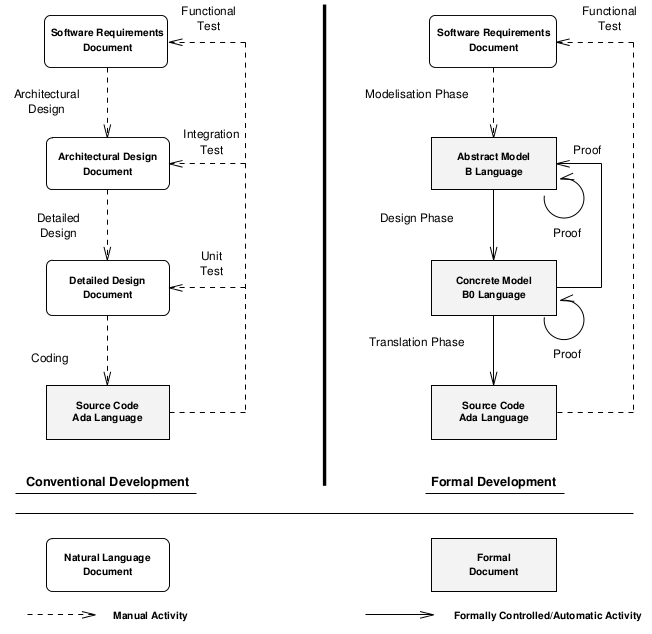
\includegraphics[scale=0.70]{ressources/formal_dev.png}
\caption{\label{DifferentsCycles}
Cycle de développement formel vs cycle conventionnel~\cite[page 374]{behm1999meteor}.}
\end{figure}

\section{Exemples d'utilisation de la méthode B}

\emph{La première application réellement industrielle a été la ligne METEOR (ligne 14) du métro parisien mise en service en octobre 1998. D'autres lignes de métro ont suivi un peu partout dans le monde. Pour fixer les idées, l'un des logiciels critiques d'un des systèmes de transport a nécessité 40 000 lignes B, 160 000 lignes de code ADA, environ 44 000 obligations de preuve B dont 1 300 ont eu besoin d'une démonstration interactive (non automatique) et une centaine de règles ajoutées.}\cite{dossierTechnique}

\subsection{Diffusion de la méthode B}
\emph{Dans tous les secteurs industriels ont été développées les notions très voisines de SIL (Safety Integrity Level) dans le domaine du transport ferroviaire et de l’industrie, d’ASIL (Automotive Safety Integrity Level ) dans le domaine automobile ou de DAL (Development Assurance Level) dans le domaine aéronautique. Un SIL est lié au niveau de confiance que l'on peut avoir dans un système. Ce niveau de confiance est associé au niveau de qualité du processus de conception/réalisation pour éviter les erreurs systématiques (principalement pour le logiciel ou des circuits intégrés complexes) et est associé à un niveau de probabilité par heure (et par ensemble) d'obtenir une défaillance contraire à la sécurité pour les erreurs aléatoires (principalement pour le matériel).}\cite{dossierTechnique}

\emph{Un processus de conception/réalisation est caractérisé par une organisation, des méthodes, des outils et des techniques spécifiques pour répondre au niveau de confiance exigé. Plus un logiciel est critique, plus on doit disposer d'une organisation robuste et des méthodes et outils qui permettent d'éviter les erreurs ou de les détecter si elles apparaissent malgré tout. Par exemple, dans le secteur ferroviaire, la norme EN50128 précise que pour un logiciel SIL3 et SIL4, les méthodes formelles sont hautement recommandées, et cela a tendance à se généraliser à l'ensemble du monde industriel.}\cite{dossierTechnique}

La \cref{UtilisationB} présente la diffusion de la méthode B pour les systèmes logiciels SIL4.
\begin{figure}[h]
\centering
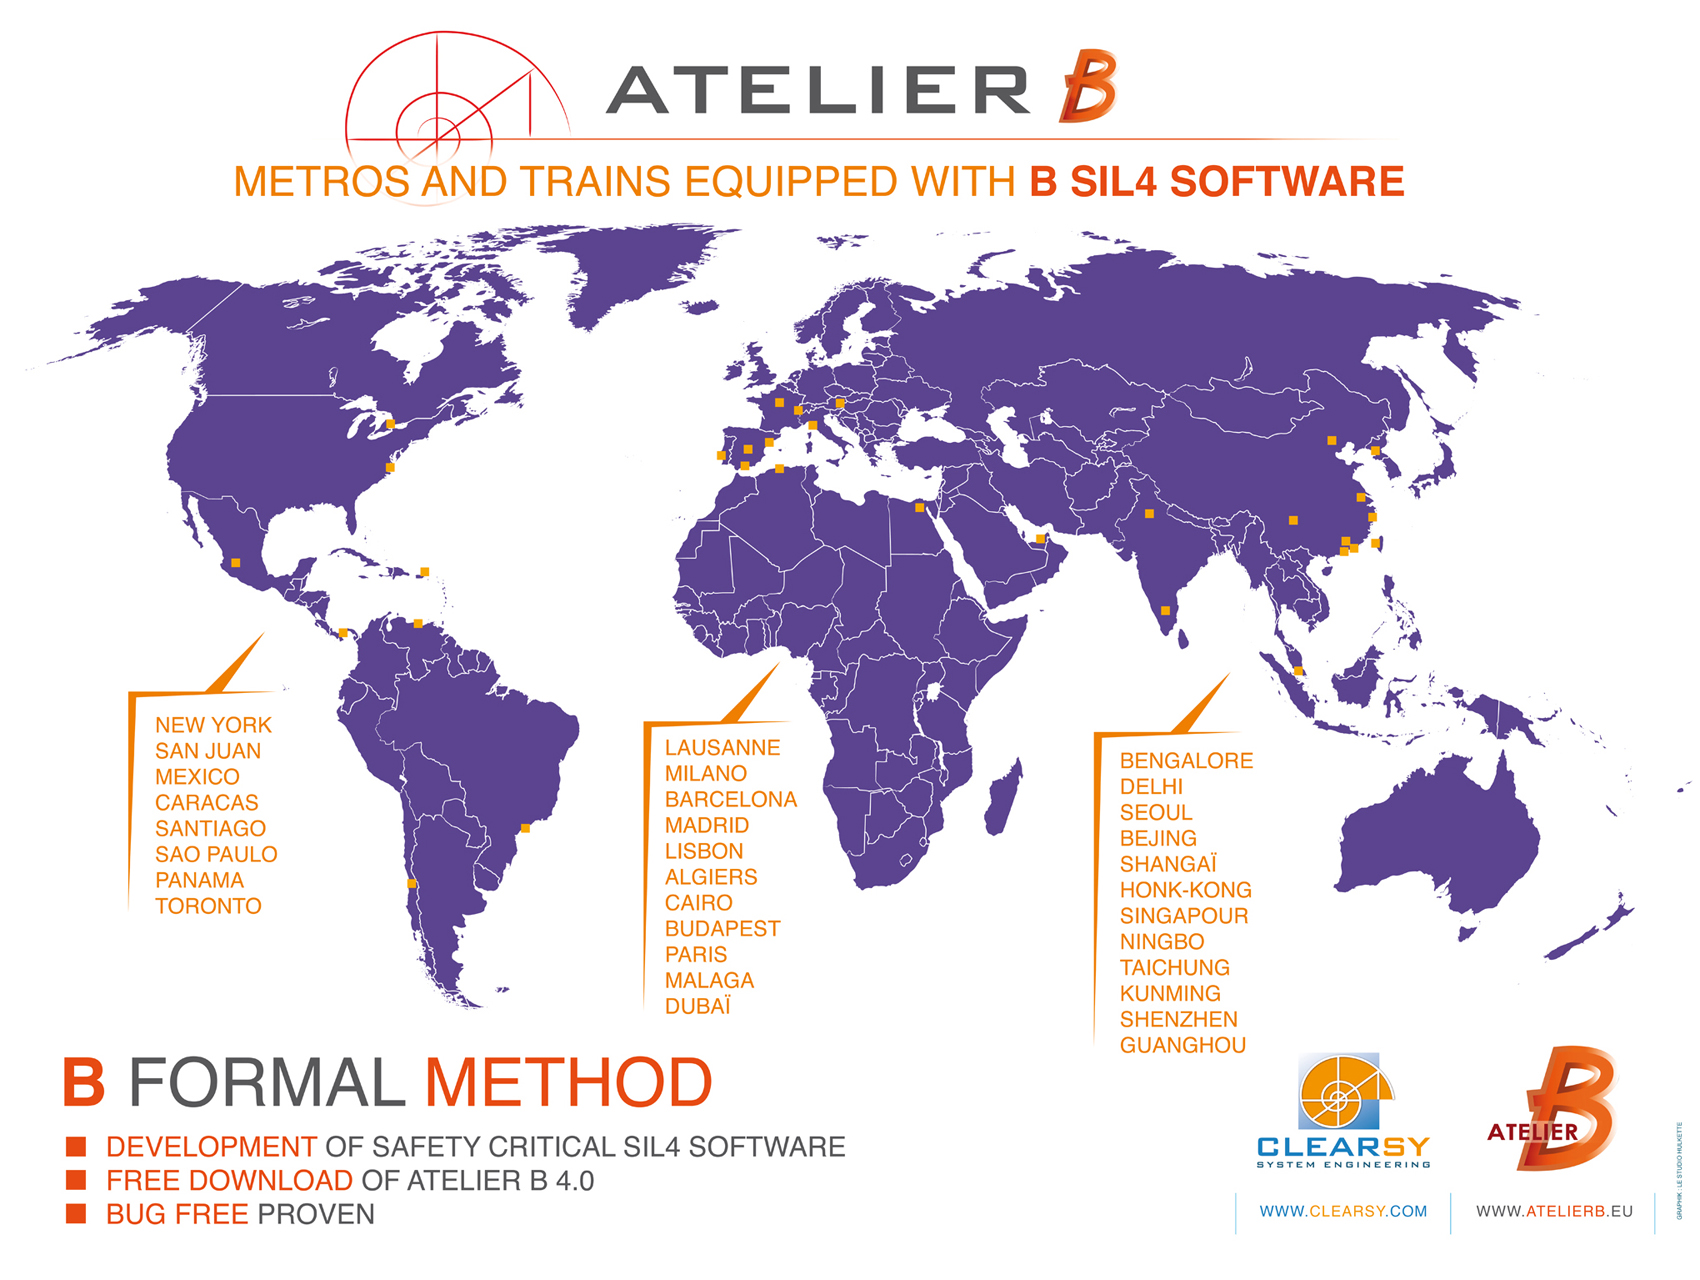
\includegraphics[scale=0.23]{ressources/carte-monde-projets-b.jpg}
\caption{\label{UtilisationB}Diffusion de la méthode B. Image provenant de \url{http://www.methode-b.com/methode-formelle}}
\end{figure}



\section{B événementiel et programme}

Au milieu des années 90, une extension de la méthode B a été développée afin d'étudier non seulement des systèmes logiciels mais aussi des systèmes événementiels représentés sous forme de systèmes à transitions.

\emph{Une machine en B  événementiel, n'a pas des opérations qui seront appelées par d'autres opérations, mais des  événements. Un  événement est spécifié comme une opération gardée. Un événement  est une transition qu'on peut observer.\newline
\indent Un  événement est déclenché lorsque sa garde est vérifiée. Si plusieurs événements sont déclenchables (i.e. leur garde est vérifiée), le déclenchement est indéterminisme. \newline
\indent Quand on raffine, alors qu'en B classique on affaiblit les préconditions, en B événementiel, on renforce les gardes.}\cite{habrias2006specifications}

Les preuves a réaliser diffèrent du B \og normal\fg. Par exemple il faut :
\begin{itemize}
\item prouver que l'état initial vérifie l'invariant pour l'état initial $x$; $ Init \Rightarrow I(x)$
\item prouver que tous les événements respectent les invariants : $ I(x) \wedge P(e)(x, x') \Rightarrow I(x')$ où $BA(e)(x, x')$ sont les prédicats associés à événement $e$ sur l'état initial $x$ et l'état final $x'$.
\item prouver l'absence de deadlock (i.e. une garde est toujours vérifiée) : $ I(x) \Rightarrow \left( grd(e_1) \vee \ldots grd(e_n) \right)$
\end{itemize}

\iffalse
In the last two subsections, we have introduced B models following the classification
into two main categories abstract machines and models; both are called components
but they are not dealing with the same approach. We detail structuring mechanisms
of both approaches to be complete on references of work 

Abstract machines are based on classical mechanisms like the call of operation or the
input/output mechanisms. On the other hand, reactive systems react to the environ-
ment with respect to external stimuli; abstract models of the event-based B approach
intend to integrate the reactivity to stimuli by promoting events rather than opera-
tions.
Contrary to operations, events have no parameters and there is no access to
state variables. At most one event is observed at any time of the system.

An (abstract) model is made up of a part defining mathematical structures
related to the problem to solve and a part containing elements on state variables,
transitions and (safety and invariance) properties of the model. Proof obligations
are generated from the model to ensure that properties are effectively holding: it
is called internal consistency of the model. A model is assumed to be closed and
it means that every possible change over state variables is defined by transitions;
transitions correspond to events observed by the specifier.
page 19


La preuve de cohérence porte
notamment sur la préservation de l'invariant, comme nous l’avons
vu en B classique, complétée par deux autres preuves : la preuve
de faisabilité et la preuve de vivacité.\cite{dossierTechnique}
\fi

\appendix

\section{Théorie ZFC}
\label{ZFC}
La théorie des ensembles de Zermelo est publiée en 1908 et instaure une axiomatique pour formuler une théorie moderne des ensembles qui n'est pas confrontée aux paradoxes de la théorie de Cantor (par exemple, le paradoxe lié à l'existence d'un ensemble qui contiendrait tous les ensembles).

En 1922, Fraenkel et Skolem ajoutent des axiomes et le système en résultant est connu sous le nom de théorie de Zermelo-Fraenkel, abrégé en ZF.

L'axiome du choix, déjà présent dans la théorie d'origine de Zermelo est souvent rajouté séparément.

On utilise la logique du premier ordre.

\subsection{Théorie de Zermelo (Z)}

\begin{axiom}[Axiome d'extensionnalité] Cet axiome définit l'égalité entre ensemble comme l'égalité de leurs éléments.
\begin{align}
\forall A\ \forall B \
\left[ 
\forall x \left( x \in A \Leftrightarrow x \in B  \right) \Rightarrow A = B
\right] 
\end{align}
\end{axiom}

\begin{axiom}[Axiome de la paire] Cet axiome définit, à partir deux ensemble A et B, un nouvel ensemble paire contenant A et B exactement.
\begin{align}
\forall A \ \forall B \ \exists C \forall x \left[ x \in C \Leftrightarrow \left( x = A \vee x = B \right) \right]
\end{align}
\end{axiom}

\begin{axiom}[Axiome de la réunion] Cet axiome définit, à partir d'un ensemble A, un nouvel ensemble $\bigcup A$ contenant les éléments des éléments de A. Avec l'axiome de la paire on peut définir l'union avec $A \cup B = \bigcup \left\{A, B\right\}$.
\begin{align}
\forall A\ \exists B\ \forall C\ \left( C\in B \Leftrightarrow \exists D\ \left( D\in A \wedge C\in D \right) \right)
\end{align}
\end{axiom}


\begin{axiom}[Schéma d'axiomes de compréhension] Aussi appelé, schéma d'axiomes de séparation, il permet de définir la construction d'ensembles en compréhension. Étant donné un ensemble $A$ et une propriété $\varphi$, il affirme l'existence de l'ensemble B des éléments de A vérifiant la propriété $\varphi$.

Ainsi, pour toute propriété $\varphi$ ne contenant pas d'autre variable libre que $x, a_1 \ldots a_p$ on définit l'axiome suivant :
\begin{align}
\forall a_1 \ldots a_n \ \forall A \ \exists B \ \forall x \ \left( x \in B \Leftrightarrow \left[ x \in A \wedge \varphi \left(x, a_1, \ldots, a_n \right) \right] \right) 
\end{align}
\end{axiom}

\begin{axiom}[Axiome de l'infini] Cet axiome définit qu'il existe un ensemble auquel appartient l'ensemble vide et qui est clos par application du successeur$ x \rightarrow x \cup \{x\}$. Il permet ainsi de construire un ensemble qui contient une représentation des entiers naturels. On note que l'ensemble vide existe comme conséquence de la logique du premier ordre du schéma d'axiomes de compréhension.
\begin{align}
\exists A \left( \emptyset \in A \land \forall x (x \in A \Rightarrow x \cup \{x\} \in A) \right) 
\end{align}
\end{axiom}

\begin{axiom}[Axiome de l'ensemble des parties] Cet axiome définit que pour tout ensemble $A$ il existe un ensemble auquel appartiennent exactement tous les sous-ensembles de $A$.
\begin{align}
\forall A \ \exists P \ \forall B \left[B \in P \Leftrightarrow \forall C \left( C \in B \Rightarrow C \in A \right) \right] 
\end{align}
\end{axiom}

On note ici que l'axiome de l'existence de l'ensemble vide n'est pas mentionné car il peut aussi être introduit à partir de la logique du premier ordre du schéma d'axiomes de compréhension.

Dès qu'il existe un ensemble, l'existence de l'ensemble vide peut être démontrée par compréhension, comme étant le sous-ensemble des éléments de celui-ci qui vérifient une propriété toujours fausse.
Or, en logique du premier ordre, les domaines d'interprétation des variables d'objets de base, ici des variables d'ensemble, sont non vides, ce qui permet donc de prouver l'existence de l'ensemble vide.

De plus, l'unicité de l'ensemble vidé découle de l'axiome d'extensionnalité.

\subsection{Théorie de Zermelo-Fraenkel (ZF)}

La théorie ZF ajoute deux axiomes à l'axiomatique déjà présentée.

\begin{axiom}[Axiome de fondation] Tout ensemble non vide x possède un élément y tel que x et y soit disjoint.
\begin{align}
\forall x [ \exists a ( a \in x) \Rightarrow \exists y ( y \in x \land \lnot \exists z (z \in y \land z \in x))]. 
\end{align}
\end{axiom}

\begin{axiom}[Schéma d'axiomes de remplacement] Ce schéma étend le schéma d'axiomes de compréhension de la théorie de Zermelo. Il définit que un ensemble A étant donné, son image par une relation fonctionnelle est un ensemble.

Ainsi, pour toute propriété $\phi$ ne contenant pas d'autre variable libre que $x, y, a_1 \ldots a_p$ on définit l'axiome suivant :
\begin{align}
\forall A \ \forall a_1 \forall \ a_2 \ldots \forall a_n \ 
\bigl[ \forall x ( x\in A \Rightarrow \exists! y\,\phi ) \Rightarrow \exists B \ \forall x \bigl(x\in A \Rightarrow \exists y (y\in B \land \phi) \bigr) \bigr]
\end{align}
\end{axiom}

\subsection{Théorie de Zermelo-Fraenkel avec axiome du choix (ZFC)}

\begin{axiom}[Axiome du choix] Étant donné un ensemble X d'ensembles non vides, il existe une fonction définie sur X, appelée fonction de choix, qui à chacun d'entre eux associe un de ses éléments.
\begin{align}
\forall X \left[ \emptyset \notin X \Rightarrow \exists f: X \rightarrow \bigcup X, \quad \forall A \in X \, ( f(A) \in A ) \right] \,. 
\end{align}
\end{axiom}

\section{Logique de Hoare pour la preuve de programmes}
\label{Hoare}

Les règles d'inférences de Hoare\footnote{Une partie de ces règles proviennent de \url{http://www.pps.univ-paris-diderot.fr/~kesner/enseignement/master1/gl/hoare-4.pdf}.} permettent la construction de programmes devant être appelés avec certaines préconditions et garantissant certaines postconditions.

\begin{axiom}[Règle de la conditionnelle]
On note $P[E/x]$ l'expression $P$ dans laquelle les occurrences libres de la variable $x$ ont été remplacées par l'expression $E$.
\begin{align}
\frac{}{\{P[E/x]\}\ x:=E \ \{P\} }
\end{align}
\end{axiom}

\begin{axiom}[Règle de la composition séquentielle]
\begin{align}
\frac {\{P\}\ S\ \{Q\}\ , \ \{Q\}\ T\ \{R\} } {\{P\}\ S;T\ \{R\}}
\end{align}
\end{axiom}

\begin{axiom}[Règle de la conditionnel]
\begin{align}
\frac { \{B \wedge P\}\ S\ \{Q\}\ ,\ \{\neg B \wedge P \}\ T\ \{Q\} } { \{P\}\ \textbf{si}\ B\ \textbf{alors}\ S\ \textbf{sinon}\ T\ \textbf{finsi}\ \{Q\} }
\end{align}
\end{axiom}

\begin{axiom}[Règle de l'itération (boucle while)]
\begin{align}
\frac { \{Inv \wedge C \}\ S\ \{Inv \} } { \{Inv \}\ \textbf{tant que}\ C\ \textbf{faire}\ S\ \textbf{fait}\ \{Inv \wedge \neg C \} }
\end{align}
\end{axiom}

\begin{axiom}[Règle de conséquence]
\begin{align}
\frac { P^\prime \rightarrow\ P\ ,\ \lbrace P \rbrace\ S\ \lbrace Q \rbrace\ ,\ Q \rightarrow\ Q^\prime } { \lbrace P^\prime\ \rbrace\ S\ \lbrace Q^\prime\rbrace }
\end{align}
\end{axiom}

On peut prouver la correction totale à condition de prouver la terminaison des boucles.
Pour se faire, il faut et il suffit qu'il existe une relation $<$ bien fondée (i.e. il n'existe pas de suite infinie $(x_n)$ d'éléments telle qu'on ait $\forall n, \ x_{n+1} < x_n$), et une expression $V$ appelée variant, dont la valeur décroit strictement à chaque itération de la boucle.

\begin{axiom}[Règle de l'itération avec terminaison]
\begin{align}
\frac{< \textrm{\ est\ bien fondée},\;\{Inv \land C \land V=z \}\;S\;\{Inv \land V < z\}} {\textrm{la boucle suivante termine}, \{Inv\}\;\textbf{tant que}\;C\; \textbf{faire}\; S \ \textbf{fait} \;\{Inv \land \lnot C \} }
\end{align}
\end{axiom}
%\mathbf{tant que}

\section{Syntaxe des prédicats et des expressions}
\label{SyntaxPredicatExpression}
\begin{itemize}
\item Prédicat
\begin{itemize}
\item Prédicat $\wedge$ Prédicat
\item Prédicat $\Rightarrow$ Prédicat
\item $\lnot$ Prédicat
\item $\exists$ Variable • Prédicat
\item [Variable := Expression] Prédicat
\item Expression = Expression
\item Expression $\in$ Set
\end{itemize}
\item Expression
\begin{itemize}
\item Variable
\item $[$Variable := Expression$]$Expression
\item Expression, Expression
\item Set
\item Variable
\item Identificateur
\item Variable, Variable
\end{itemize}
\item Set
\item Set $\times$ Set
\item P(Set)
\item choice(Set)
\item \{Variable $|$ Prédicat\}
\item BIG

\end{itemize}

\section{Compléments syntaxiques du langage B}
\label{ComplementSyntaxique}
\subsection{Autres clauses des machines abstraites}

\textbf{ASSERTIONS} : Propriété logique dérivée des invariants, contraintes et propriétés. Étant dérivées, i.e. induites par le reste, il n'est pas nécessaire de les démontrer - et même, elles n'impliquent a priori pas réciproquement le reste. En revanche, elles facilitent le travail du prouveur automatique.

\textbf{DEFINITIONS} : Alias facilitant la rédaction du reste de la machine.

TODO : $ABSTRACT\_CONSTANTS$, $CONCRETE\_VARIABLES$

\section{Code source de l'exemple}
\label{CodeSource}
Cette annexe contient le code source associé à l'exemple donné à la~\cref{ExempleComplet}, page~\pageref{ExempleComplet}.

\paragraph{Code source de la machine abstraite}
\begin{verbatim}
MACHINE
    utils
OPERATIONS
res <-- mini(xx,yy) =
    PRE
        xx : NAT &
        yy : NAT
    THEN
        res := min ({xx,yy})
    END;
res <--maxi(xx,yy,zz) =
    PRE
        xx : NAT &
        yy : NAT &
        zz : NAT
    THEN
        res := max({xx,yy,zz})
    END
END
\end{verbatim}

\paragraph{Code source de l'implémentation}
\begin{verbatim}
IMPLEMENTATION
   utils_i
REFINES
   utils
OPERATIONS
res <-- mini ( xx , yy ) =
    IF
        xx >= yy
    THEN
        res:= yy
    ELSE
        res := xx
    END;
res <--maxi ( xx , yy , zz ) =
    BEGIN
    IF
        xx >= yy
    THEN
        res := xx
    END;
    IF
        xx <= yy
    THEN
        res := yy
    END;
    IF
        res <= zz
    THEN
        res := zz
    END
    END
END
\end{verbatim}

% ===================================
% Bib
\bibliographystyle{plain}
\bibliography{biblio.bib}
% ===================================

\end{document}